\documentclass[twoside]{book}

% Packages required by doxygen
\usepackage{fixltx2e}
\usepackage{calc}
\usepackage{doxygen}
\usepackage[export]{adjustbox} % also loads graphicx
\usepackage{graphicx}
\usepackage[utf8]{inputenc}
\usepackage{makeidx}
\usepackage{multicol}
\usepackage{multirow}
\PassOptionsToPackage{warn}{textcomp}
\usepackage{textcomp}
\usepackage[nointegrals]{wasysym}
\usepackage[table]{xcolor}

% Font selection
\usepackage[T1]{fontenc}
\usepackage[scaled=.90]{helvet}
\usepackage{courier}
\usepackage{amssymb}
\usepackage{sectsty}
\renewcommand{\familydefault}{\sfdefault}
\allsectionsfont{%
  \fontseries{bc}\selectfont%
  \color{darkgray}%
}
\renewcommand{\DoxyLabelFont}{%
  \fontseries{bc}\selectfont%
  \color{darkgray}%
}
\newcommand{\+}{\discretionary{\mbox{\scriptsize$\hookleftarrow$}}{}{}}

% Page & text layout
\usepackage{geometry}
\geometry{%
  a4paper,%
  top=2.5cm,%
  bottom=2.5cm,%
  left=2.5cm,%
  right=2.5cm%
}
\tolerance=750
\hfuzz=15pt
\hbadness=750
\setlength{\emergencystretch}{15pt}
\setlength{\parindent}{0cm}
\setlength{\parskip}{3ex plus 2ex minus 2ex}
\makeatletter
\renewcommand{\paragraph}{%
  \@startsection{paragraph}{4}{0ex}{-1.0ex}{1.0ex}{%
    \normalfont\normalsize\bfseries\SS@parafont%
  }%
}
\renewcommand{\subparagraph}{%
  \@startsection{subparagraph}{5}{0ex}{-1.0ex}{1.0ex}{%
    \normalfont\normalsize\bfseries\SS@subparafont%
  }%
}
\makeatother

% Headers & footers
\usepackage{fancyhdr}
\pagestyle{fancyplain}
\fancyhead[LE]{\fancyplain{}{\bfseries\thepage}}
\fancyhead[CE]{\fancyplain{}{}}
\fancyhead[RE]{\fancyplain{}{\bfseries\leftmark}}
\fancyhead[LO]{\fancyplain{}{\bfseries\rightmark}}
\fancyhead[CO]{\fancyplain{}{}}
\fancyhead[RO]{\fancyplain{}{\bfseries\thepage}}
\fancyfoot[LE]{\fancyplain{}{}}
\fancyfoot[CE]{\fancyplain{}{}}
\fancyfoot[RE]{\fancyplain{}{\bfseries\scriptsize Generated by Doxygen }}
\fancyfoot[LO]{\fancyplain{}{\bfseries\scriptsize Generated by Doxygen }}
\fancyfoot[CO]{\fancyplain{}{}}
\fancyfoot[RO]{\fancyplain{}{}}
\renewcommand{\footrulewidth}{0.4pt}
\renewcommand{\chaptermark}[1]{%
  \markboth{#1}{}%
}
\renewcommand{\sectionmark}[1]{%
  \markright{\thesection\ #1}%
}

% Indices & bibliography
\usepackage{natbib}
\usepackage[titles]{tocloft}
\setcounter{tocdepth}{3}
\setcounter{secnumdepth}{5}
\makeindex

% Hyperlinks (required, but should be loaded last)
\usepackage{ifpdf}
\ifpdf
  \usepackage[pdftex,pagebackref=true]{hyperref}
\else
  \usepackage[ps2pdf,pagebackref=true]{hyperref}
\fi
\hypersetup{%
  colorlinks=true,%
  linkcolor=blue,%
  citecolor=blue,%
  unicode%
}

% Custom commands
\newcommand{\clearemptydoublepage}{%
  \newpage{\pagestyle{empty}\cleardoublepage}%
}

\usepackage{caption}
\captionsetup{labelsep=space,justification=centering,font={bf},singlelinecheck=off,skip=4pt,position=top}

%===== C O N T E N T S =====

\begin{document}

% Titlepage & ToC
\hypersetup{pageanchor=false,
             bookmarksnumbered=true,
             pdfencoding=unicode
            }
\pagenumbering{roman}
\begin{titlepage}
\vspace*{7cm}
\begin{center}%
{\Large beginner\+\_\+tutorials \\[1ex]\large 1.\+0 }\\
\vspace*{1cm}
{\large Generated by Doxygen 1.8.11}\\
\end{center}
\end{titlepage}
\clearemptydoublepage
\tableofcontents
\clearemptydoublepage
\pagenumbering{arabic}
\hypersetup{pageanchor=true}

%--- Begin generated contents ---
\chapter{This is beginners tutorial for creating a simple R\+OS package}
\label{index}\hypertarget{index}{}\input{index}
\chapter{beginner\+\_\+tutorials}
\label{md_README}
\hypertarget{md_README}{}
\href{https://github.com/RajPShinde/begineer_tutorials/blob/master/LICENSE}{\tt } \href{https://github.com/RajPShinde/begineer_tutorials/blob/master/docs}{\tt }

\subsection*{Authors}

{\bfseries Raj Prakash Shinde} -\/ \href{https://github.com/RajPShinde}{\tt Git\+Hub} ~\newline
I am a Masters in Robotics Engineering student at the University of Maryland, College Park. My primary area of interest are Legged Robotics and Automation.

\subsection*{Overview}

This is beginners tutorial for creating a simple R\+OS package called begineers\+\_\+tutorials with a Publisher \& Subscriber node. Where a publisher named talker, publishes a message and the subscriber called, listener hears the message. The message type here is a string. A talker node has a service that can be used to change the message content. A launch file can be used to launch both the nodes, which also passes the loop rate as an argument.

\subsection*{Dependencies}


\begin{DoxyEnumerate}
\item Ubuntu 16.\+04
\item R\+OS Kinetic
\end{DoxyEnumerate}

\subsection*{Build}

Steps to build 
\begin{DoxyCode}
1 mkdir -p ~/catkin\_ws/src
2 cd ~/catkin\_ws/
3 catkin\_make
4 source devel/setup.bash
5 cd src/
6 git clone https://github.com/RajPShinde/beginner\_tutorials
7 cd ~/catkin\_ws/
8 catkin\_make
\end{DoxyCode}


\subsection*{Run}


\begin{DoxyEnumerate}
\item Launch both nodes Individually Run roscore (Open a Terminal) 
\begin{DoxyCode}
1 cd ~/catkin\_ws/
2 source ./devel/setup.bash
3 roscore
\end{DoxyCode}
 Run talker node (Open a new Terminal) 
\begin{DoxyCode}
1 cd ~/catkin\_ws/
2 source ./devel/setup.bash
3 rosrun beginner\_tutorials talker 10
\end{DoxyCode}
 Run listener node (Open a new Terminal) 
\begin{DoxyCode}
1 cd ~/catkin\_ws/
2 source ./devel/setup.bash
3 rosrun beginner\_tutorials listener
\end{DoxyCode}

\item Launch both nodes with the launchfile (Open a new Terminal) 
\begin{DoxyCode}
1 cd ~/catkin\_ws/
2 source ./devel/setup.bash
3 roslaunch beginner\_tutorials nodelauncher.launch
\end{DoxyCode}
 You can change the frequency by passing an argumnet, default is 10 (Open a new Terminal) 
\begin{DoxyCode}
1 cd ~/catkin\_ws/
2 source ./devel/setup.bash
3 roslaunch beginner\_tutorials nodelauncher.launch rate:=8
\end{DoxyCode}

\item Run service to change string launch both nodes and then Open a new Terminal 
\begin{DoxyCode}
1 cd ~/catkin\_ws/
2 source ./devel/setup.bash
3 rosservice call /service\_string "Enter new string"
\end{DoxyCode}

\item To view Log levels using rqt console and rqt logger level Open a new Terminal 
\begin{DoxyCode}
1 rosrun rqt\_console rqt\_console
\end{DoxyCode}
 Open a new Terminal 
\begin{DoxyCode}
1 rosrun rqt\_logger\_level rqt\_logger\_level
\end{DoxyCode}

\item Inspecting TF Frames After launching both nodes using launch file, we can inspect the TF frames using tf\+\_\+echo and rqt\+\_\+tf\+\_\+tree (Open a new Terminal)
\end{DoxyEnumerate}


\begin{DoxyCode}
1 rosrun tf tf\_echo /world /talk
\end{DoxyCode}
 To genereate a pdf of tf frame 
\begin{DoxyCode}
1 rosrun tf view\_frames
\end{DoxyCode}
 Open a new Terminal 
\begin{DoxyCode}
1 rosrun rqt\_tf\_tree rqt\_tf\_tree
\end{DoxyCode}



\begin{DoxyEnumerate}
\item Run Test Open a new Terminal 
\begin{DoxyCode}
1 cd ~/catkin\_ws
2 source ./devel/setup.bash
3 catkin\_make run\_tests\_beginner\_tutorials
4 rostest beginner\_tutorials testlauncher.launch
\end{DoxyCode}

\item Record in Rosbag To record in a rosbag, pass a true argument to the launch file(\+Open a new Terminal) 
\begin{DoxyCode}
1 roslaunch beginner\_tutorials nodelauncher.launch recordbag:=true
\end{DoxyCode}
 To avoid recording, either pass false or don\textquotesingle{}t pass any argument 
\begin{DoxyCode}
1 roslaunch beginner\_tutorials nodelauncher.launch recordbag:=false
\end{DoxyCode}
 OR 
\begin{DoxyCode}
1 roslaunch beginner\_tutorials nodelauncher.launch
\end{DoxyCode}

\item Use Rosbag First launch the listener node and then Open a new Terminal and play rosbag 
\begin{DoxyCode}
1 cd ~/catkin\_ws/src/beginner\_tutorials/results
2 rosbag play recording.bag
\end{DoxyCode}
 You can see that the listener node can hear the rosbag data of previously recorded talker node.
\end{DoxyEnumerate}

\subsection*{Reference}


\begin{DoxyItemize}
\item \href{http://wiki.ros.org/}{\tt http\+://wiki.\+ros.\+org/} 
\end{DoxyItemize}
\chapter{Class Index}
\section{Class List}
Here are the classes, structs, unions and interfaces with brief descriptions\+:\begin{DoxyCompactList}
\item\contentsline{section}{\hyperlink{struct_x}{X} }{\pageref{struct_x}}{}
\end{DoxyCompactList}

\chapter{File Index}
\section{File List}
Here is a list of all documented files with brief descriptions\+:\begin{DoxyCompactList}
\item\contentsline{section}{src/\hyperlink{listener_8cpp}{listener.\+cpp} \\*R\+OS Subscriber Node }{\pageref{listener_8cpp}}{}
\item\contentsline{section}{src/\hyperlink{talker_8cpp}{talker.\+cpp} \\*R\+OS Publisher Node }{\pageref{talker_8cpp}}{}
\item\contentsline{section}{test/\hyperlink{main_8cpp}{main.\+cpp} \\*Main for testing }{\pageref{main_8cpp}}{}
\item\contentsline{section}{test/\hyperlink{test_talker_8cpp}{test\+Talker.\+cpp} \\*Tests for \hyperlink{talker_8cpp}{talker.\+cpp} }{\pageref{test_talker_8cpp}}{}
\end{DoxyCompactList}

\chapter{Class Documentation}
\hypertarget{struct_x}{}\section{X Struct Reference}
\label{struct_x}\index{X@{X}}
\subsection*{Public Attributes}
\begin{DoxyCompactItemize}
\item 
\hyperlink{talker_8cpp_a0ba76bcac54e80d914f29f0c76d947be}{std\+::string} {\bfseries temp}\hypertarget{struct_x_a08b1cca1250e07bb26e61316d0dd8ac3}{}\label{struct_x_a08b1cca1250e07bb26e61316d0dd8ac3}

\end{DoxyCompactItemize}


The documentation for this struct was generated from the following file\+:\begin{DoxyCompactItemize}
\item 
src/\hyperlink{talker_8cpp}{talker.\+cpp}\end{DoxyCompactItemize}

\chapter{File Documentation}
\hypertarget{listener_8cpp}{}\section{src/listener.cpp File Reference}
\label{listener_8cpp}\index{src/listener.\+cpp@{src/listener.\+cpp}}


R\+OS Subscriber Node.  


{\ttfamily \#include $<$ros/ros.\+h$>$}\\*
{\ttfamily \#include $<$std\+\_\+msgs/\+String.\+h$>$}\\*
Include dependency graph for listener.\+cpp\+:
\nopagebreak
\begin{figure}[H]
\begin{center}
\leavevmode
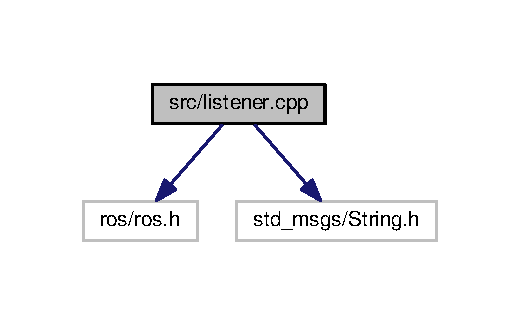
\includegraphics[width=250pt]{listener_8cpp__incl}
\end{center}
\end{figure}
\subsection*{Functions}
\begin{DoxyCompactItemize}
\item 
void \hyperlink{listener_8cpp_ae5c0c11b4a60030ee8df1a3ae0b6f758}{chatter\+Callback} (const std\+\_\+msgs\+::\+String\+::\+Const\+Ptr \&msg)
\begin{DoxyCompactList}\small\item\em function to print L\+OG message on terminal \end{DoxyCompactList}\item 
int \hyperlink{listener_8cpp_a3c04138a5bfe5d72780bb7e82a18e627}{main} (int argc, char $\ast$$\ast$argv)
\begin{DoxyCompactList}\small\item\em Main function for Subscriber. \end{DoxyCompactList}\end{DoxyCompactItemize}


\subsection{Detailed Description}
R\+OS Subscriber Node. 

\begin{DoxyCopyright}{Copyright}
M\+IT License, © 2019 Raj Shinde
\end{DoxyCopyright}
\begin{DoxyAuthor}{Author}
Raj Shinde 
\end{DoxyAuthor}
\begin{DoxyDate}{Date}
11/10/2019 
\end{DoxyDate}
\begin{DoxyVersion}{Version}
1.\+0 
\end{DoxyVersion}
\hypertarget{test_talker_8cpp_DESCRIPTION}{}\subsection{D\+E\+S\+C\+R\+I\+P\+T\+I\+ON}\label{test_talker_8cpp_DESCRIPTION}
A Subscriber node that subscibes to talker 

\subsection{Function Documentation}
\index{listener.\+cpp@{listener.\+cpp}!chatter\+Callback@{chatter\+Callback}}
\index{chatter\+Callback@{chatter\+Callback}!listener.\+cpp@{listener.\+cpp}}
\subsubsection[{\texorpdfstring{chatter\+Callback(const std\+\_\+msgs\+::\+String\+::\+Const\+Ptr \&msg)}{chatterCallback(const std_msgs::String::ConstPtr &msg)}}]{\setlength{\rightskip}{0pt plus 5cm}void chatter\+Callback (
\begin{DoxyParamCaption}
\item[{const std\+\_\+msgs\+::\+String\+::\+Const\+Ptr \&}]{msg}
\end{DoxyParamCaption}
)}\hypertarget{listener_8cpp_ae5c0c11b4a60030ee8df1a3ae0b6f758}{}\label{listener_8cpp_ae5c0c11b4a60030ee8df1a3ae0b6f758}


function to print L\+OG message on terminal 


\begin{DoxyParams}{Parameters}
{\em std\+\_\+msgs\+::\+String\+::\+Const\+Ptr\&} & published string \\
\hline
\end{DoxyParams}
\begin{DoxyReturn}{Returns}
None 
\end{DoxyReturn}
\index{listener.\+cpp@{listener.\+cpp}!main@{main}}
\index{main@{main}!listener.\+cpp@{listener.\+cpp}}
\subsubsection[{\texorpdfstring{main(int argc, char $\ast$$\ast$argv)}{main(int argc, char **argv)}}]{\setlength{\rightskip}{0pt plus 5cm}int main (
\begin{DoxyParamCaption}
\item[{int}]{argc, }
\item[{char $\ast$$\ast$}]{argv}
\end{DoxyParamCaption}
)}\hypertarget{listener_8cpp_a3c04138a5bfe5d72780bb7e82a18e627}{}\label{listener_8cpp_a3c04138a5bfe5d72780bb7e82a18e627}


Main function for Subscriber. 


\begin{DoxyParams}{Parameters}
{\em argc} & no of argumnets \\
\hline
{\em argv} & char pointer consisting arguments \\
\hline
\end{DoxyParams}
\begin{DoxyReturn}{Returns}
0 
\end{DoxyReturn}

\hypertarget{talker_8cpp}{}\section{src/talker.cpp File Reference}
\label{talker_8cpp}\index{src/talker.\+cpp@{src/talker.\+cpp}}


R\+OS Publisher Node.  


{\ttfamily \#include $<$ros/ros.\+h$>$}\\*
{\ttfamily \#include $<$std\+\_\+msgs/\+String.\+h$>$}\\*
{\ttfamily \#include $<$tf/transform\+\_\+broadcaster.\+h$>$}\\*
{\ttfamily \#include $<$sstream$>$}\\*
{\ttfamily \#include $<$string$>$}\\*
{\ttfamily \#include \char`\"{}beginner\+\_\+tutorials/service\+String.\+h\char`\"{}}\\*
Include dependency graph for talker.\+cpp\+:
\nopagebreak
\begin{figure}[H]
\begin{center}
\leavevmode
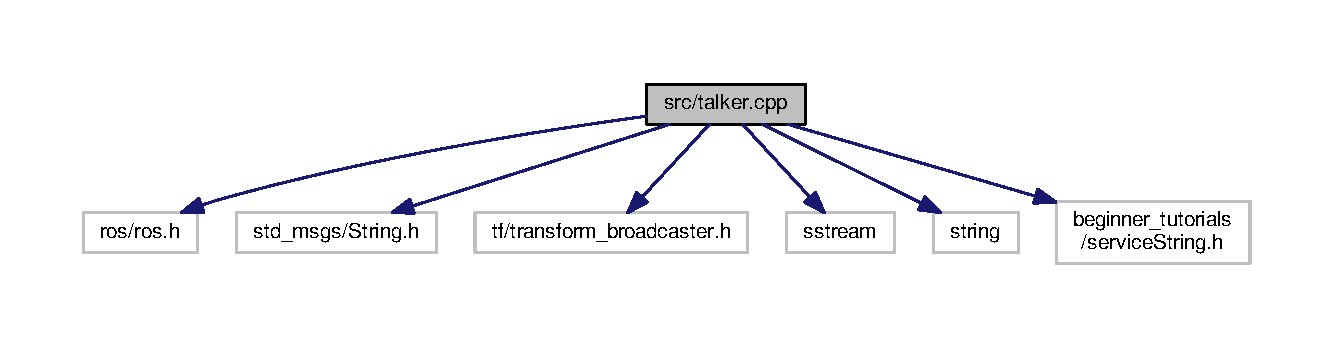
\includegraphics[width=350pt]{talker_8cpp__incl}
\end{center}
\end{figure}
\subsection*{Classes}
\begin{DoxyCompactItemize}
\item 
struct \hyperlink{struct_x}{X}
\end{DoxyCompactItemize}
\subsection*{Functions}
\begin{DoxyCompactItemize}
\item 
bool \hyperlink{talker_8cpp_a0ba76bcac54e80d914f29f0c76d947be}{string} (beginner\+\_\+tutorials\+::service\+String\+::\+Request \&req, beginner\+\_\+tutorials\+::service\+String\+::\+Response \&res)
\begin{DoxyCompactList}\small\item\em Function to provide service functionality. \end{DoxyCompactList}\item 
int \hyperlink{talker_8cpp_a3c04138a5bfe5d72780bb7e82a18e627}{main} (int argc, char $\ast$$\ast$argv)
\begin{DoxyCompactList}\small\item\em Main function for Publisher. \end{DoxyCompactList}\end{DoxyCompactItemize}
\subsection*{Variables}
\begin{DoxyCompactItemize}
\item 
struct \hyperlink{struct_x}{X} {\bfseries t}\hypertarget{talker_8cpp_a713043a7f1ef60dd29454fe66fb0db59}{}\label{talker_8cpp_a713043a7f1ef60dd29454fe66fb0db59}

\end{DoxyCompactItemize}


\subsection{Detailed Description}
R\+OS Publisher Node. 

\begin{DoxyCopyright}{Copyright}
M\+IT License, © 2019 Raj Shinde
\end{DoxyCopyright}
\begin{DoxyAuthor}{Author}
Raj Shinde 
\end{DoxyAuthor}
\begin{DoxyDate}{Date}
11/10/2019 
\end{DoxyDate}
\begin{DoxyVersion}{Version}
1.\+0 
\end{DoxyVersion}
\hypertarget{test_talker_8cpp_DESCRIPTION}{}\subsection{D\+E\+S\+C\+R\+I\+P\+T\+I\+ON}\label{test_talker_8cpp_DESCRIPTION}
A Publisher node that publishes tf frame 

\subsection{Function Documentation}
\index{talker.\+cpp@{talker.\+cpp}!main@{main}}
\index{main@{main}!talker.\+cpp@{talker.\+cpp}}
\subsubsection[{\texorpdfstring{main(int argc, char $\ast$$\ast$argv)}{main(int argc, char **argv)}}]{\setlength{\rightskip}{0pt plus 5cm}int main (
\begin{DoxyParamCaption}
\item[{int}]{argc, }
\item[{char $\ast$$\ast$}]{argv}
\end{DoxyParamCaption}
)}\hypertarget{talker_8cpp_a3c04138a5bfe5d72780bb7e82a18e627}{}\label{talker_8cpp_a3c04138a5bfe5d72780bb7e82a18e627}


Main function for Publisher. 


\begin{DoxyParams}{Parameters}
{\em argc} & no of argumnets \\
\hline
{\em argv} & char pointer consisting arguments \\
\hline
\end{DoxyParams}
\begin{DoxyReturn}{Returns}
0 
\end{DoxyReturn}
\index{talker.\+cpp@{talker.\+cpp}!string@{string}}
\index{string@{string}!talker.\+cpp@{talker.\+cpp}}
\subsubsection[{\texorpdfstring{string(beginner\+\_\+tutorials\+::service\+String\+::\+Request \&req, beginner\+\_\+tutorials\+::service\+String\+::\+Response \&res)}{string(beginner_tutorials::serviceString::Request &req, beginner_tutorials::serviceString::Response &res)}}]{\setlength{\rightskip}{0pt plus 5cm}bool string (
\begin{DoxyParamCaption}
\item[{beginner\+\_\+tutorials\+::service\+String\+::\+Request \&}]{req, }
\item[{beginner\+\_\+tutorials\+::service\+String\+::\+Response \&}]{res}
\end{DoxyParamCaption}
)}\hypertarget{talker_8cpp_a0ba76bcac54e80d914f29f0c76d947be}{}\label{talker_8cpp_a0ba76bcac54e80d914f29f0c76d947be}


Function to provide service functionality. 


\begin{DoxyParams}{Parameters}
{\em beginner\+\_\+tutorials\+::service\+String\+::\+Request} & Request argument \\
\hline
{\em beginner\+\_\+tutorials\+::service\+String\+::\+Response} & Response argumnet \\
\hline
\end{DoxyParams}
\begin{DoxyReturn}{Returns}
true 
\end{DoxyReturn}

\hypertarget{main_8cpp}{}\section{test/main.cpp File Reference}
\label{main_8cpp}\index{test/main.\+cpp@{test/main.\+cpp}}


Main for testing.  


{\ttfamily \#include $<$ros/ros.\+h$>$}\\*
{\ttfamily \#include $<$gtest/gtest.\+h$>$}\\*
Include dependency graph for main.\+cpp\+:
\nopagebreak
\begin{figure}[H]
\begin{center}
\leavevmode
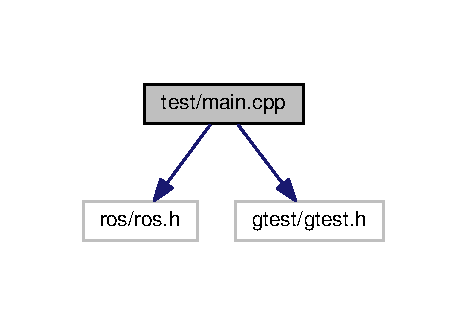
\includegraphics[width=224pt]{main_8cpp__incl}
\end{center}
\end{figure}
\subsection*{Functions}
\begin{DoxyCompactItemize}
\item 
int \hyperlink{main_8cpp_a3c04138a5bfe5d72780bb7e82a18e627}{main} (int argc, char $\ast$$\ast$argv)
\begin{DoxyCompactList}\small\item\em Main for testing. \end{DoxyCompactList}\end{DoxyCompactItemize}


\subsection{Detailed Description}
Main for testing. 

\begin{DoxyCopyright}{Copyright}
M\+IT License, © 2019 Raj Shinde
\end{DoxyCopyright}
\begin{DoxyAuthor}{Author}
Raj Shinde 
\end{DoxyAuthor}
\begin{DoxyDate}{Date}
11/10/2019 
\end{DoxyDate}
\begin{DoxyVersion}{Version}
1.\+0 
\end{DoxyVersion}
\hypertarget{test_talker_8cpp_DESCRIPTION}{}\subsection{D\+E\+S\+C\+R\+I\+P\+T\+I\+ON}\label{test_talker_8cpp_DESCRIPTION}
All the test are run 

\subsection{Function Documentation}
\index{main.\+cpp@{main.\+cpp}!main@{main}}
\index{main@{main}!main.\+cpp@{main.\+cpp}}
\subsubsection[{\texorpdfstring{main(int argc, char $\ast$$\ast$argv)}{main(int argc, char **argv)}}]{\setlength{\rightskip}{0pt plus 5cm}int main (
\begin{DoxyParamCaption}
\item[{int}]{argc, }
\item[{char $\ast$$\ast$}]{argv}
\end{DoxyParamCaption}
)}\hypertarget{main_8cpp_a3c04138a5bfe5d72780bb7e82a18e627}{}\label{main_8cpp_a3c04138a5bfe5d72780bb7e82a18e627}


Main for testing. 


\begin{DoxyParams}{Parameters}
{\em argc} & no of argumnets \\
\hline
{\em argv} & char pointer consisting arguments \\
\hline
\end{DoxyParams}
\begin{DoxyReturn}{Returns}
R\+U\+N\+\_\+\+A\+L\+L\+\_\+\+T\+E\+S\+T\+S() 
\end{DoxyReturn}

\hypertarget{test_talker_8cpp}{}\section{test/test\+Talker.cpp File Reference}
\label{test_talker_8cpp}\index{test/test\+Talker.\+cpp@{test/test\+Talker.\+cpp}}


Tests for \hyperlink{talker_8cpp}{talker.\+cpp}.  


{\ttfamily \#include $<$gtest/gtest.\+h$>$}\\*
{\ttfamily \#include $<$ros/ros.\+h$>$}\\*
{\ttfamily \#include $<$tf/transform\+\_\+listener.\+h$>$}\\*
{\ttfamily \#include $<$ros/service\+\_\+client.\+h$>$}\\*
{\ttfamily \#include $<$std\+\_\+msgs/\+String.\+h$>$}\\*
{\ttfamily \#include \char`\"{}beginner\+\_\+tutorials/service\+String.\+h\char`\"{}}\\*
Include dependency graph for test\+Talker.\+cpp\+:
\nopagebreak
\begin{figure}[H]
\begin{center}
\leavevmode
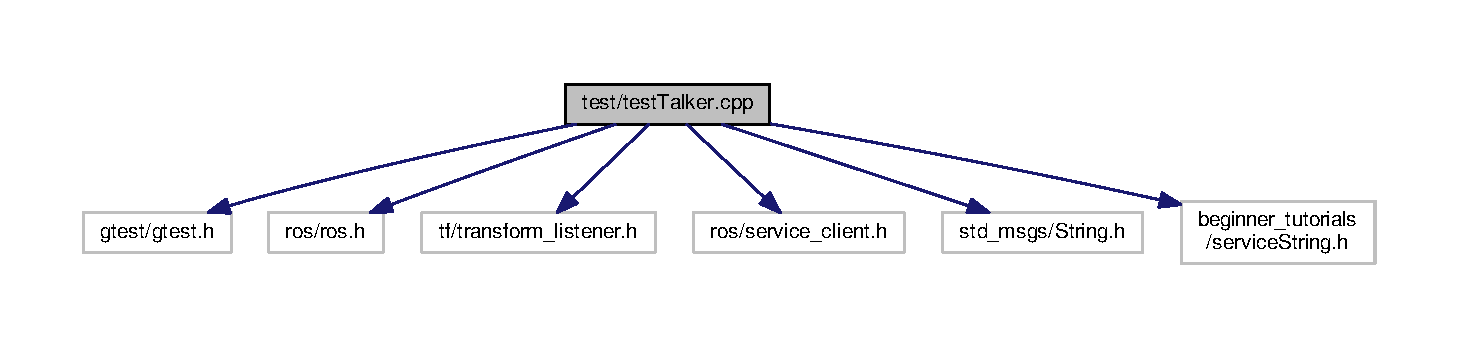
\includegraphics[width=350pt]{test_talker_8cpp__incl}
\end{center}
\end{figure}
\subsection*{Functions}
\begin{DoxyCompactItemize}
\item 
\hyperlink{test_talker_8cpp_ad8615bc0b2081ca6485dfd376534ff9f}{T\+E\+ST} (Talker, test\+Service)\hypertarget{test_talker_8cpp_ad8615bc0b2081ca6485dfd376534ff9f}{}\label{test_talker_8cpp_ad8615bc0b2081ca6485dfd376534ff9f}

\begin{DoxyCompactList}\small\item\em A unit test to check that the talker string service works correctly. \end{DoxyCompactList}\item 
\hyperlink{test_talker_8cpp_a82b5792955d05743b5a07645e2221544}{T\+E\+ST} (Talker, test\+Tf)\hypertarget{test_talker_8cpp_a82b5792955d05743b5a07645e2221544}{}\label{test_talker_8cpp_a82b5792955d05743b5a07645e2221544}

\begin{DoxyCompactList}\small\item\em A unit test to check the Broadcasted frames offset. \end{DoxyCompactList}\end{DoxyCompactItemize}


\subsection{Detailed Description}
Tests for \hyperlink{talker_8cpp}{talker.\+cpp}. 

\begin{DoxyCopyright}{Copyright}
M\+IT License, © 2019 Raj Shinde
\end{DoxyCopyright}
\begin{DoxyAuthor}{Author}
Raj Shinde 
\end{DoxyAuthor}
\begin{DoxyDate}{Date}
11/10/2019 
\end{DoxyDate}
\begin{DoxyVersion}{Version}
1.\+0 
\end{DoxyVersion}
\hypertarget{test_talker_8cpp_DESCRIPTION}{}\subsection{D\+E\+S\+C\+R\+I\+P\+T\+I\+ON}\label{test_talker_8cpp_DESCRIPTION}
Test are written for talker node 
%--- End generated contents ---

% Index
\backmatter
\newpage
\phantomsection
\clearemptydoublepage
\addcontentsline{toc}{chapter}{Index}
\printindex

\end{document}
